\section{Planlægning og test af programmet}

Planen som blev lagt de første dage i projektet blev egentlig fulgt ganske godt igennem projektet. De første dage blev brugt på brainstorming og planlægning af, hvordan vi ønskede at vores spil skulle se ud, og hvilke features som skulle inkluderes. De tekniske specifikationer er et resultat deraf. I overlappet på design og brainstorm delen blev forskellige dele af projektet delt ud, sådan at hver enkel gruppemedlem kom med et udkast til design af forskellige dele af programmet.
\begin{figure}[h]
\begin{center}
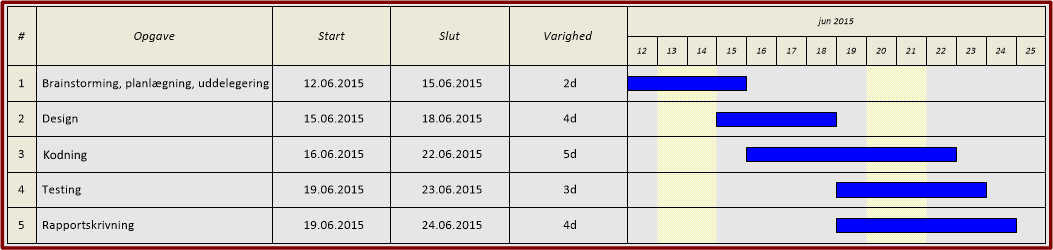
\includegraphics[scale=0.7]{img/Gantt_Chart.png}
\caption{Gantt chart af vores plan}
\end{center}
\end{figure}
 Igennem designfasen blev der kigget på flowcharts, samt skrevet pseudokode. Hen mod slutningen af designfasen blev der skrevet mere og mere reel kode. Kodeskrivningen og testing delen følger hinanden. Sidst i kodefasen blev vi nød til at droppe et af de mål vi havde sat os for at overholde planen, som vi havde lagt og blive færdig med projektet.  De sidste dage op mod deadline blev der skrevet rapport.
\subsection{Problemer}
Under udarbejdelsen af programmet havde vi problemer, som vi ikke havde forudset under design-fasen, vi vil her gennemgå nogle af dem der voldte os mest besvær, at debugge.
\subsubsection{Problemer med realloc}
\label{reallocfejl}
I designfasen havde vi forestillet os at vores boxstruct blot skulle være skrevet som i \textbf{newBoxStack()}, hvor vi dog kun allokerede plads til et enkelt element i hvert array. Ydermere skulle der være en variabel kaldet capacity, der betegnede hvor stort stacket var. Vi ville derefter i \textbf{createBoxes()} undersøge om \textit{*(box).capacity} == \textit{*(box).size} , og hvis det var sandt allokere yderlige 10 pladser med realloc. Dette fungerede dog ikke, og boksene fik tilfældige lokationer på banen. Vi mistænker at der ikke var plads til at dynamisk allokere plads på boardet og finde sammenhængende plads i rammene, og det derfor gik galt. Hvis vi i stedet startede med at allokere plads, gav det os ikke problemer.
\subsubsection{Problemer med knapperne}
Vi havde problemer med knapperne på boardet: Vi var i tvivl om vores kode var dårlig, eller om det var fordi knapperne var slidte og ødelagte. Vi lavede en debouncer, og det hjalp lidt på nogle af knapperne, men vi havde stadig problemer, og nåede aldrig at komme til bunds i problemet. Vi er dog ret overbevist om at problemerne stammer fra de slidte knapper.
\subsection{Test af programmet}
Programmet blev testet op mod vores designkrav og de tekniske specifikationer. Først blev grundelementerne kodet og testet, og når det levede op til specifikationerne blev programmet udvidet med nye funktioner. Koden blev altså skrevet og testet med en buttom up metode, hvor det første element var selve banen. Derefter fulgte strikeren, samt det at kunne få strikeren til at flytte sig. Næste skridt var boldens bevægelse, samt den simple refleksion på kanterne og strikeren, hvor indgangsvinkel var lig udgangsvinkel. Så fulgte kasserne med alle deres egenskaber, og boldens refleksion på kasserne. Endeligt blev strikerens udgangsvinkel ændret alt efter indgangsvinkel. En menu blev lavet sideløbende med spillet. 
Al vores testing blev udført i terminalen, hvor programmet var sat op til at teste, i den forstand, at programmet printede informationer som vi havde  brug for. Dette gjorde vi f.eks. i forbindelse med testing af strikeren, hvor vi printede hvor bolden blev detekteret på strikeren, hvad ind- og udgangsvinklen var. Dette gjorde vi for at checke om vores program opførte sig som forventet.


